\documentclass[doc]{apa6} % Options: jou (journal), man (manuscript), doc (document)
\usepackage[american]{babel} % Set language
\usepackage{csquotes}        % Required for APA citations
\usepackage{subcaption}      % For subfigures
\usepackage{apacite}         % For APA-style references
\usepackage{graphicx}        % For including figures
\usepackage{amsmath}         % For mathematical equations
\usepackage{float}
\date{December 2024}
\usepackage{array}

\title{Predicting Student Outcomes on Standardized Testing using Machine Learning}
\shorttitle{Predicting Student Outcomes}
\author{Stacy Roberts}
\affiliation{The University of Texas at Austin}


\abstract{
Finding a solution to the problem of student success has long been a goal and a frustration in education. Helping teachers, administrators, and support staff understand which students will benefit from additional intervention to achieve successful outcomes is assumed to increase the completion rate for all students. Being able to focus on the right students most likely to need closer monitoring and more assistance in preparation helps focus public school's limited resources where they may see the highest return on investment. Accounting for co-variants outside of the school control is also necessary to understanding how best to serve the student population of a given school. This paper will focus on success in terms of standardized testing scores in Math, Reading, and Writing. Using various machine learning models, we attempt to demonstrate which machine learning models perform the best at predicting student success rates on subject testing.}

\begin{document}
\maketitle

\section{Introduction}

Predicting student outcomes is a necessary function of the public school system, which is tasked with maximizing the success of their entire student population. All schools are invested in the percentage of their students who graduate on time and go on to higher education or employment, as it is reflective of the success of the school itself. However, gaining access to student data is easier with public schools given the government mandates of public reporting they are required to follow. \cite{ecsa} This paper will focus on public school data.

There are many ideas of what types of students require more assistance to be successful in school. Focus is generally placed on socioeconomic background, race, gender, and parental education level. \cite{Bradley2022SESgap}  Time and again, higher socioeconomic areas have higher student achievement outcomes. This is true for both the high and low socioeconomic groups when the average status is higher for the area.  Higher Socioeconomic Groups have many advantages, from stable homes and plentiful food to higher quality and more stable teaching and administrative staff at the schools which service them. \cite{HSEffectsLongTerm} This paper is not intending to check all possible differentials, but does note that it is difficult to separate all the co-variant factors which contribute to the success of a student population. Is it more important to have a stable, effective teaching staff or to provide a support system where all students have stability and enough food to eat? Ideal data sets for investigating this theory would involve students of equally matched SES with large differentials in staff quality, as well as students with same teachers but large differential in SES to attempt to isolate how important SES is for student success. Since families are generally uninterested in subjecting their children to be test subjects for educational theories which may impact their success, it is very difficult to find this type of data set.

Yet there are some pockets of students who outperform expectations based on background. \cite{YanGaiLowSEG} These students often have need to finish this thought with other research

This paper aims to utilize different Machine Learning models to see if we can train and fine tune a model to predict the students who are risk of failing standardized math, reading, and writing assessments based on available background information.

\section{Research Background}
Efforts to improve student outcomes have had varying rates of success. There is no single path which guarantees that all students achieve high school graduation and beyond.  Instead, there is a continuous cycle of new research, new methods, new options to try to increase material retention, attendance, and ultimately, state testing scores.

Study after study has found that students who enter kindergarten behind their peers will struggle to make up the gap throughout their entire schooling. \cite{EdInequities} \cite{sesbehind1} \cite{sesbehind2} \cite{sesbehind3}  High quality and accessible pre-K, along with increasing availability of books at home have been shown to make significant improvements in preparing students for kindergarten. However, there are precious few resources for families on the lower and middle socioeconomic spectrum to access these trajectory changing elements for their children. \cite{cradleK} Providing more social safety nets such as paid parental leave, affordable child care, and more expanded and intensive services for families experiencing multiple adversities similar to every other developed nation would significantly improve the standing of children born into the more dire of situation.

Socioeconomic status also affects access to Twentieth century necessities like internet access and personal laptops. Given that nearly all school systems use online classrooms and school work, having access to a personal computer and internet at home is a requirement to be successful in school. However, personal computers come with a significant price tag and internet, even with income based discounts, is a monthly expense many families cannot afford.\cite{sesinternet} 

School systems focus on state testing scores as that is how they are ranked for public viewing. \cite{linnetal} These rankings then influence who chooses to buy homes within the district, which in turn influences the socioeconomic level of the population and the educational attainment and retention of the teaching, support, and admin staff attracted to said schools. The unfortunate side effect is that limited resources get reallocated to focus on preparation and support surrounding state testing, to the detriment of more holistic approaches to support the entire student. \cite{cradle}

\section{Methods and Data Analysis}
\subsection{Data Analysis}
The data selected for analysis has anonymous student information for 1000 students. It includes background information on each student with regards to parental education, reduced/free lunch, whether they completed a test preparation course, along with gender and test scores for math, reading, and writing assessments. There is enough information to make an educated guess as to the socioeconomic level of each student. Basing this classification around whether the student was on reduced/free lunch plan is substituted as a proxy for actual demographic data. Students can only qualify for the reduced/free lunch plan if their guardians are below a specified income level. While this will not correctly classify all students, based on available information it is the best method to distinguish we have accessible. Many studies base it on the mother's level of education, but this data set doesn't have that sort of granularity. \cite{maternaleducation} \cite{maternaleducation2} \cite{maternaleducation3}

The training began by performing pre-processing of the original data. Of interest was seeing if the data analysis showed any correlation between the parent's education level and the passing rates of their children. Each individualized standardized testing area was evaluated separately to see if there were different correlations for the different subjects. 

\begin{figure}[H]
    \centering
    \caption{Correlations of Parent Education to Student Scores}
    \begin{subfigure}[b]{0.28\textwidth}
    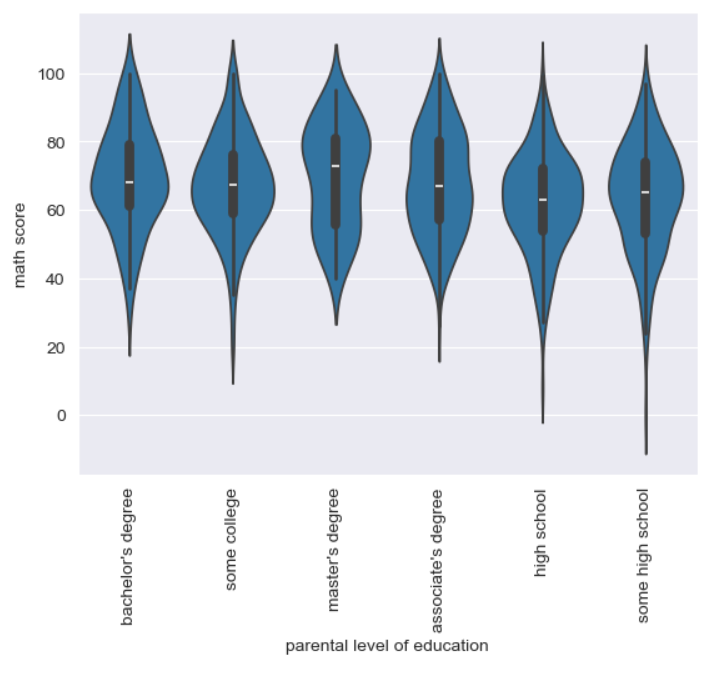
\includegraphics[width=\linewidth]{MathVsParent.png}
    \caption{Correlation of Math Scores}
    \label{fig:math}
    \end{subfigure}
    \begin{subfigure}[b]{0.28\textwidth}
    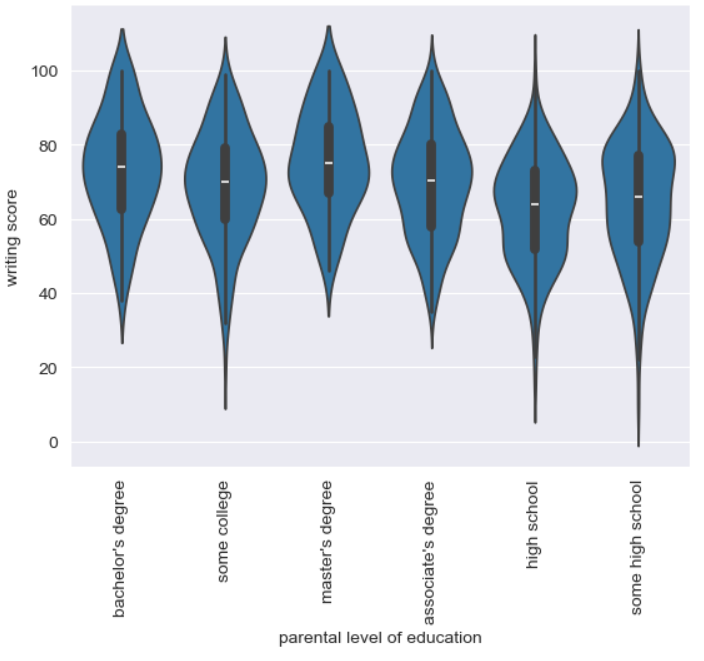
\includegraphics[width=\linewidth]{WritingVsParent.png}
    \caption{Correlation of Writing Scores}
    \label{fig:read}
    \end{subfigure}
    \begin{subfigure}[b]{0.28\textwidth}
    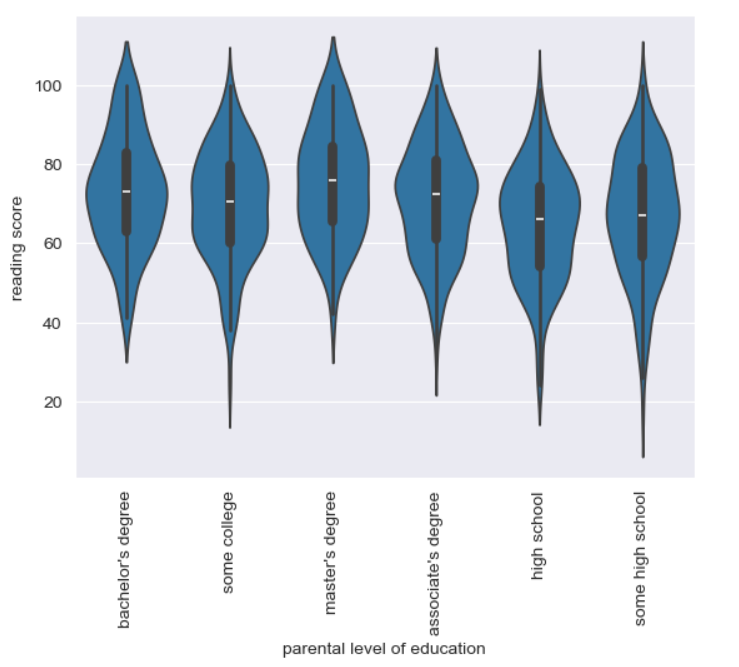
\includegraphics[width=\linewidth]{ReadingVsParent.png}
    \caption{Correlation of Reading Scores}
    \label{fig:write}
    \end{subfigure}
\end{figure}

Figure 1 indicates a small difference in outcomes between the subject areas. While the overall average isn't significantly different when looking at the data in this manner, the variance becomes noticeable as the parental education level goes down. Those students of families with the highest level of parental education also achieved the highest mean, while those whose parents only completed some high school had the widest variance in scores.

Focusing on the Math Scores chart \ref{fig:math}, while the students of all parental education levels were able to attain a similar top end score, the variability of the plot indicates a higher mean the more education the parents obtained.  Students of parents with a Master's degree had the highest mean math score, but the other education levels didn't show a significant difference in the mean.  The most noticeable difference between the categories is the lowest score rate. The lower the education level of the parents, the lower the lowest scores of the students.  Clearly there is some correlation, but not as strong of one as might be expected based on the volume of literature around SES and student success at least for this data set.
Similar to the Math score graph, the Reading and Writing scores show variability relative to parental education level.  It is more noticeable that those whose parents only achieved at or below a high school level of education had lower mean and bottom end scores in reading and writing. It would appear that within this dataset, the influence of parent's education is more noticeable in reading and writing ability than math.

It becomes more apparently how parental education level affects student performance when we compare strict pass rates, grouped by the parent's education. These graphs are normalized for the differing numbers of parents in each grouping to provide a percentage passing rate for each group.  Passing is considered achieving 70\% or higher on the standardized test.

\begin{figure}[H]
    \centering
    \caption{Correlations of Parent Education to Student Pass Rates}
    \begin{subfigure}[b]{0.28\textwidth}
    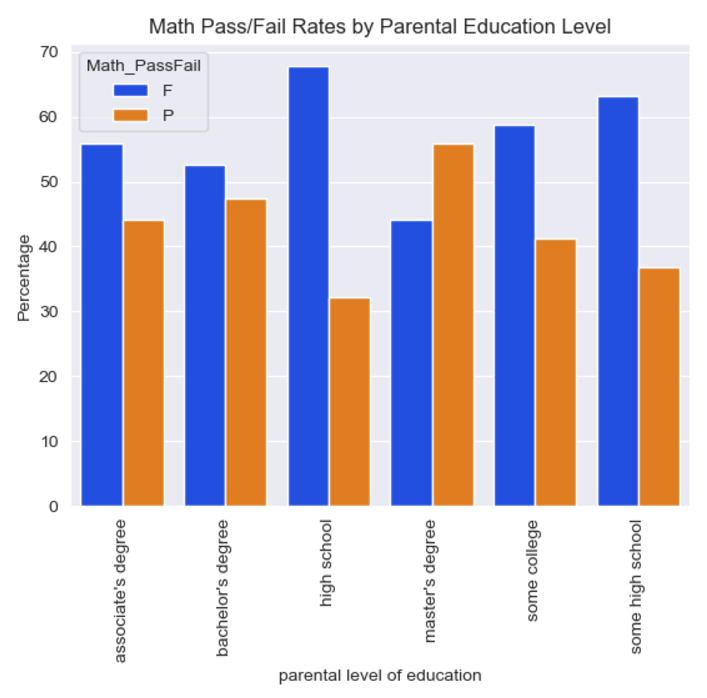
\includegraphics[width=\linewidth]{MathPFBarGraph.png}
    \caption{Passing Rates for Math Test}
    \label{fig:math}
    \end{subfigure}
    \begin{subfigure}[b]{0.28\textwidth}
    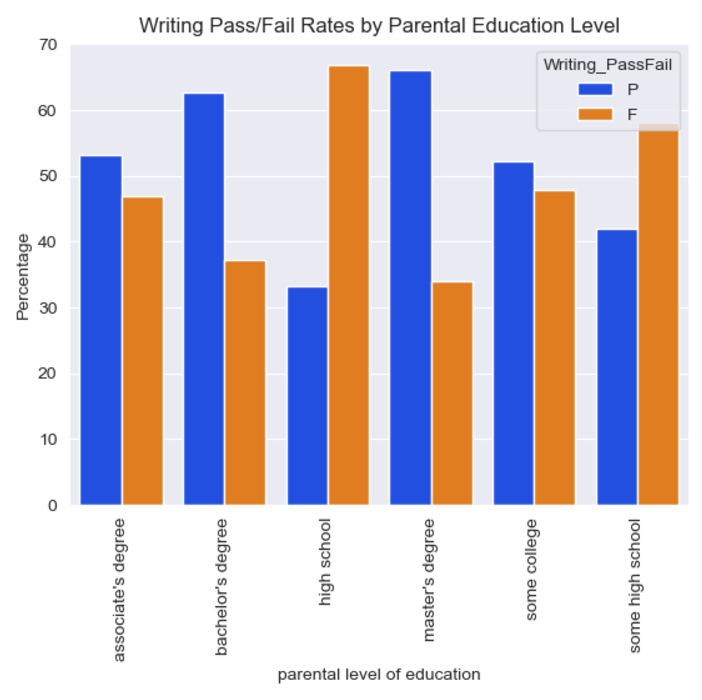
\includegraphics[width=\linewidth]{WritingPFBarGraph.png}
    \caption{Passing Rates for Writing Test}
    \label{fig:write}
    \end{subfigure}
    \begin{subfigure}[b]{0.28\textwidth}
    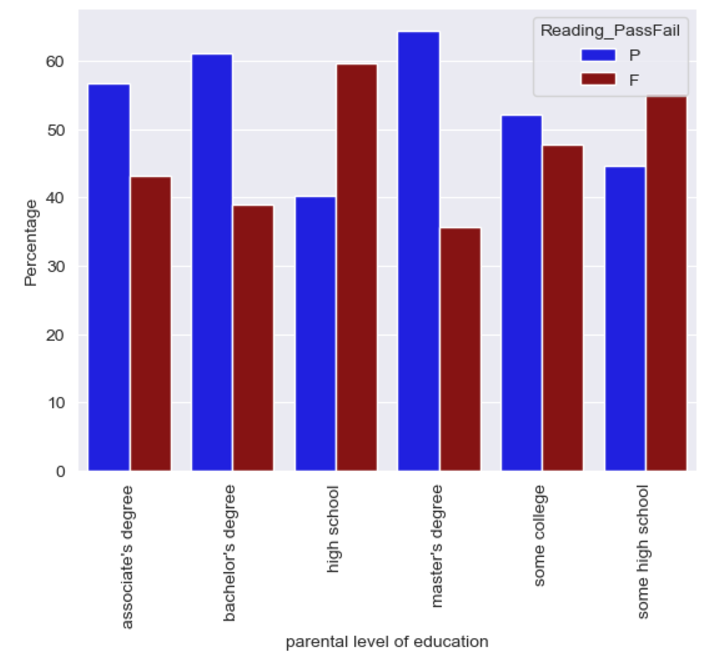
\includegraphics[width=\linewidth]{ReadingPFBarGraph.png}
    \caption{Passing Rates for Reading Test}
    \label{fig:read}
    \end{subfigure}
\end{figure}

There were much lower passing rates on the Math assessment across the board, with only students from families who obtained a Master's Degree achieving a higher than 50\% pass rate at all. In both the Writing and Reading assessments, students from families who completed some college or higher achieved a higher than 50\% pass rate with Master's Degree students having the highest success rate of all groups in both of these assessments. Based on this dataset the parental education level has an out-sized impact on Reading and Writing test ability.

If we focus only on gender, another differential becomes apparent. Female students performed better than their Male counterparts overall, and specifically in the Reading and Writing tests.  Male students performed better than Female students only in the Math test. This is regardless of parental education level.
\begin{figure}[H]
    \centering
    \caption{Average Standardized Scores by Gender}
    \begin{subfigure}[b]{0.45\textwidth}
        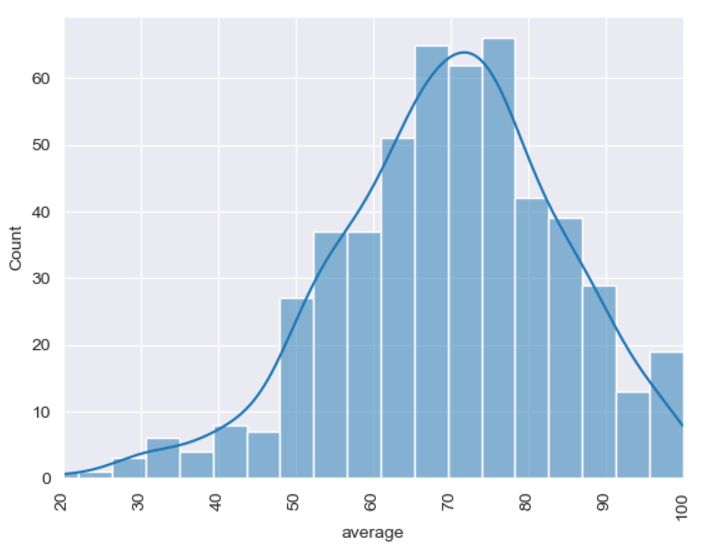
\includegraphics[width=\linewidth]{FemaleAverageScoreCurve.png}
        \caption{Female Students Avg Scores}
        \label{fig:FemaleAvg}
    \end{subfigure}
    \begin{subfigure}[b]{0.45\textwidth}
        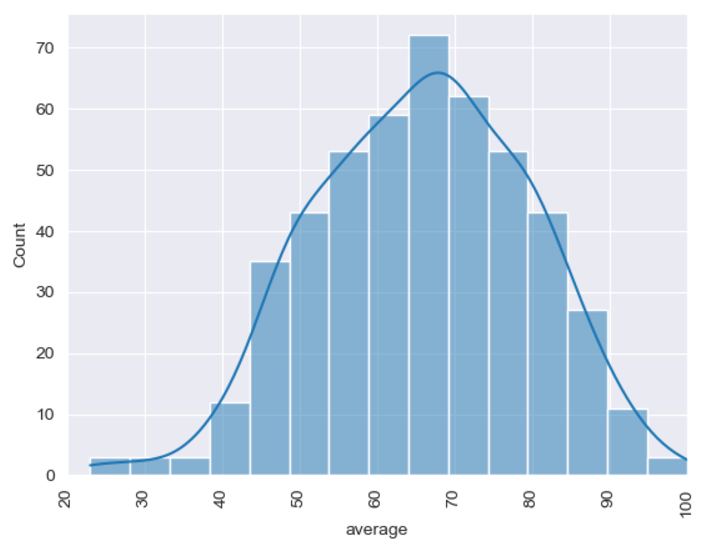
\includegraphics[width=\linewidth]{MaleAverageScoreCurve.png}
        \caption{Male Students Avg Scores}
        \label{fig:MaleAvg}
    \end{subfigure}
\end{figure}

\begin{figure}[H]
    \centering
    \caption{Math Standardized Scores by Gender}
    \begin{subfigure}[b]{0.45\textwidth}
        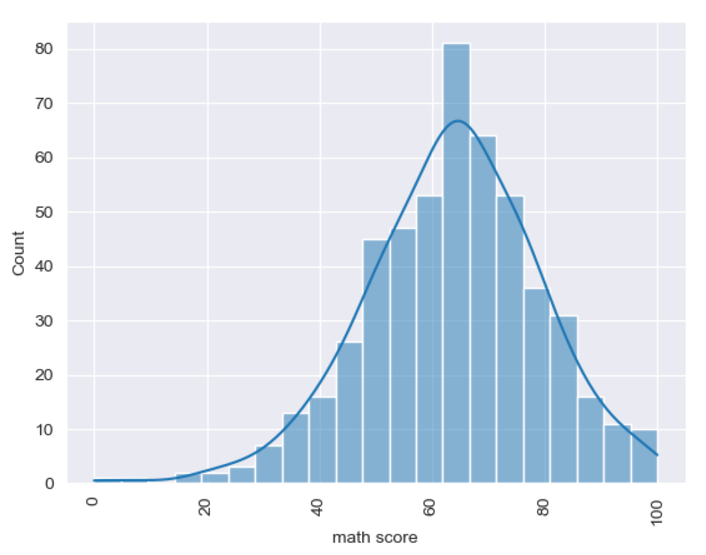
\includegraphics[width=\linewidth]{FemaleStudentsMathScoreCurve.png}
        \caption{Female Students Math Scores}
        \label{fig:FemaleMath}
    \end{subfigure}
    \begin{subfigure}[b]{0.45\textwidth}
        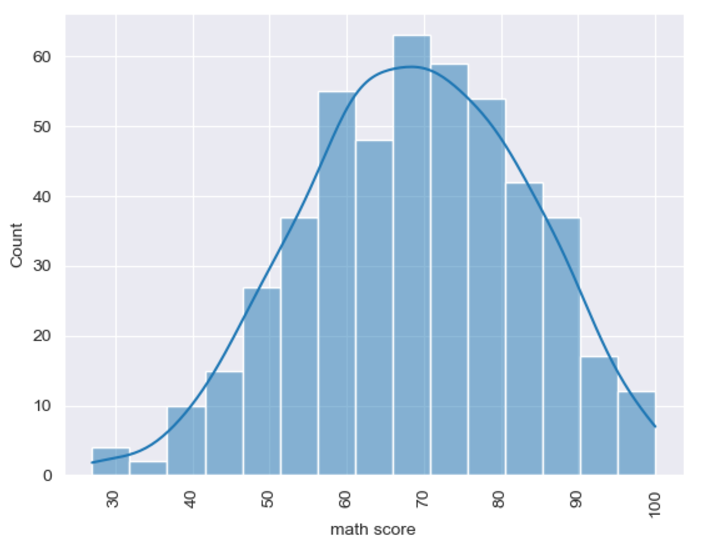
\includegraphics[width=\linewidth]{MaleStudentMathScoresCurve.png}
        \caption{Male Students Math Scores}
        \label{fig:MaleMath}
    \end{subfigure}
\end{figure}

\begin{figure}[H]
    \centering
    \caption{Writing Standardized Scores by Gender}
    \begin{subfigure}[b]{0.45\textwidth}
        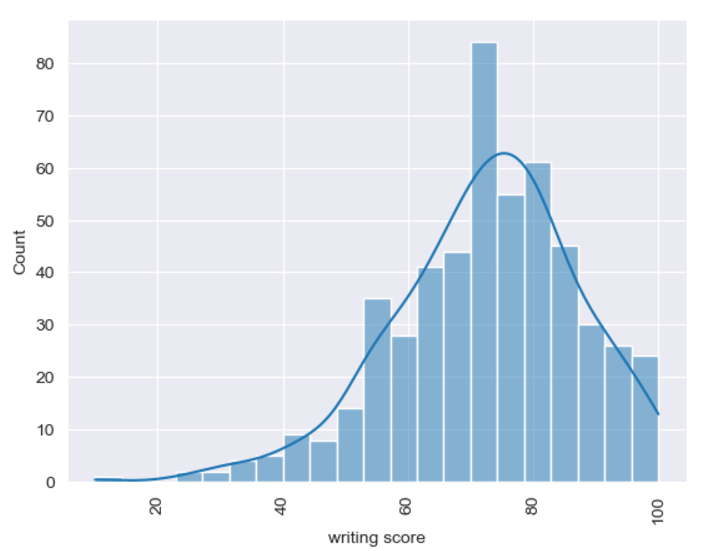
\includegraphics[width=\linewidth]{FemaleStudentsWritingScoreCurve.png}
        \caption{Female Students Writing Scores}
        \label{fig:FemaleWriting}
    \end{subfigure}
    \begin{subfigure}[b]{0.45\textwidth}
        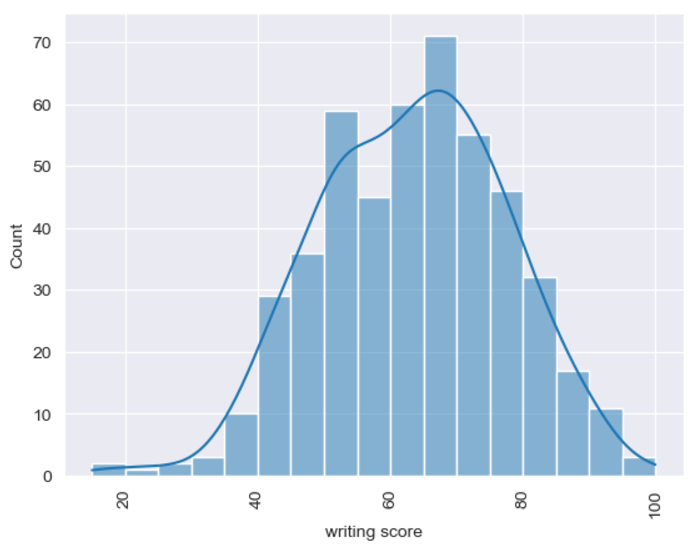
\includegraphics[width=\linewidth]{MaleStudentWritingScoreCurve.png}
        \caption{Male Students Writing Scores}
        \label{fig:MaleWriting}
    \end{subfigure}
\end{figure}
\begin{figure}[H]
    \centering
    \caption{Reading Standardized Scores by Gender}
    \begin{subfigure}[b]{0.45\textwidth}
        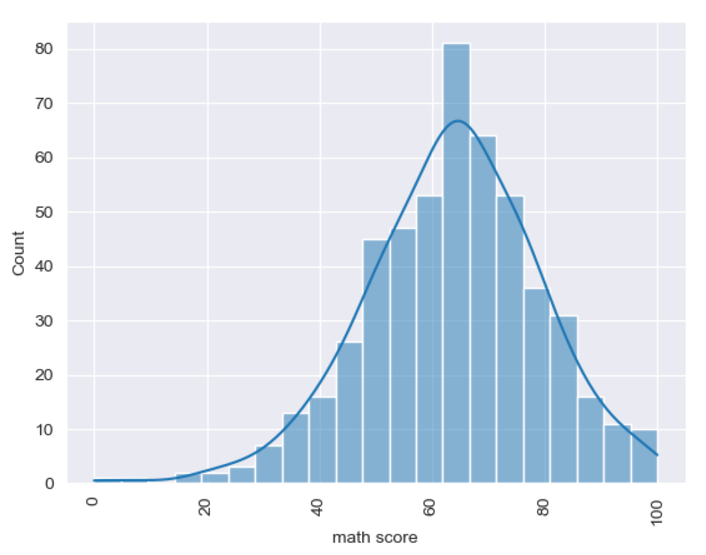
\includegraphics[width=\linewidth]{FemaleStudentsMathScoreCurve.png}
        \caption{Female Students Reading Scores}
        \label{fig:FemaleRead}
    \end{subfigure}
    \begin{subfigure}[b]{0.45\textwidth}
        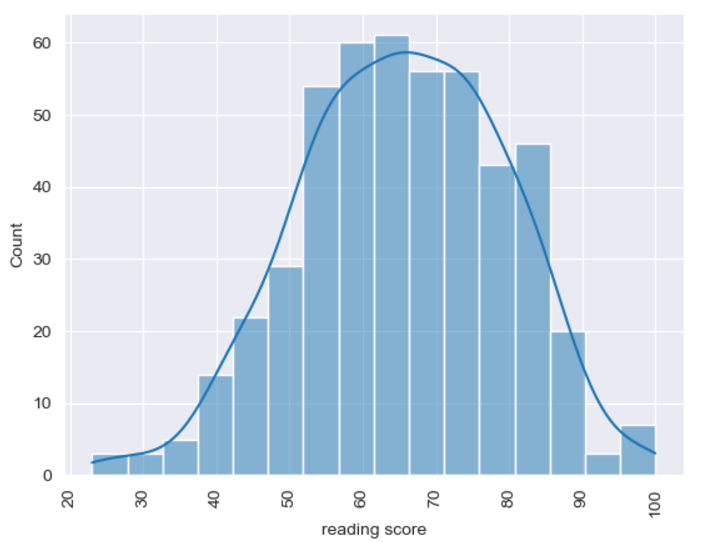
\includegraphics[width=\linewidth]{MaleStudentReadingScoreCurve.png}
        \caption{Male Students Reading Scores}
        \label{fig:MaleRead}
    \end{subfigure}
\end{figure}

Coming back to the concerns regarding student Socioeconomic Status and its impact on student performance, we invested how much the lunch program influenced the students' test scores.  Again, this is being used as another proxy for knowing the student's specific background as only students whose families earn below a specified income level are eligible for the reduced/free lunch program.

Isolating the student performance by lunch program yielded the most significant results regarding impact of family income status and student performance. Here we have only included the Average Score chart because the differential was fairly consistent across all testing subjects.

\begin{figure}[H]
    \centering
    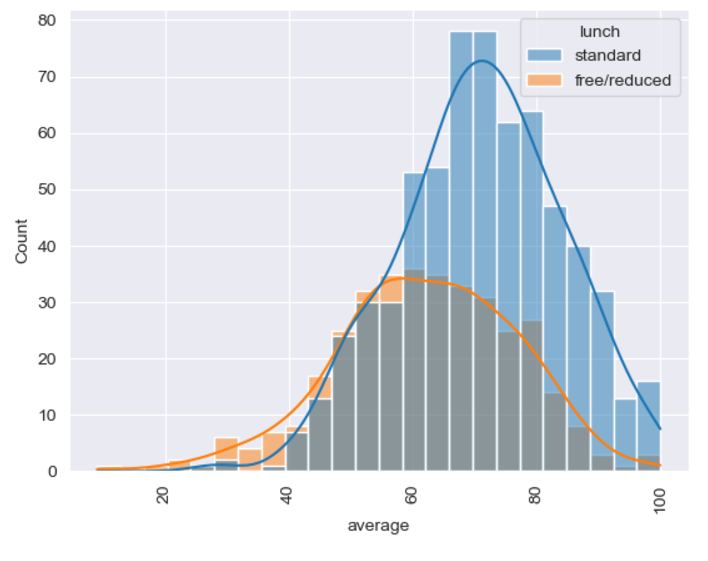
\includegraphics[width=0.75\linewidth]{StudentAvgScoresVSReducedLunch.png}
    \caption{Student Average Scores Separated by Lunch Program}
    \label{fig:lunch1}
\end{figure}
The students on the reduced/free lunch program had a mean score at least 10\% lower than those not on the plan. Also of note is the percentage of students in this dataset which were on the reduced/free lunch program. There are 1000 students total in the dataset, with 645 not on the plan and 355 on the reduced/free lunch plan. 
Investigating how Race/Ethnicity played into student success, first we need to understand how many students were in each group.

\begin{table}[H]
    \centering
    \begin{tabular}{|c|c|}
    \hline
         Group Identifier & Student Count\\
         \hline\hline
         Group A & 89\\
         \hline
         Group B & 190\\
         \hline
         Group C & 319\\
         \hline
         Group D & 262\\
         \hline
         Group E & 140\\
         \hline
    \end{tabular}
    \caption{Race/Ethnicity Student Representation Counts}
    \label{tab:RaceCount}
\end{table}
Group C is the largest represented group while Group A is the smallest. Within this limited context, we graphed the average scores of students grouped by their race/ethnicity identification. It is noteworthy that the smallest represented group, the minority, had the lowest mean of all the groups. It was also well below passing rate.  The two largest representative groups are the highest mean scores, both hovering right around the passing rate. Group B performs similarly to Group A, with a low mean below passing rate, while Group E performs the best in the set with the highest mean of all the groups. 

\begin{figure}[H]
    \centering
    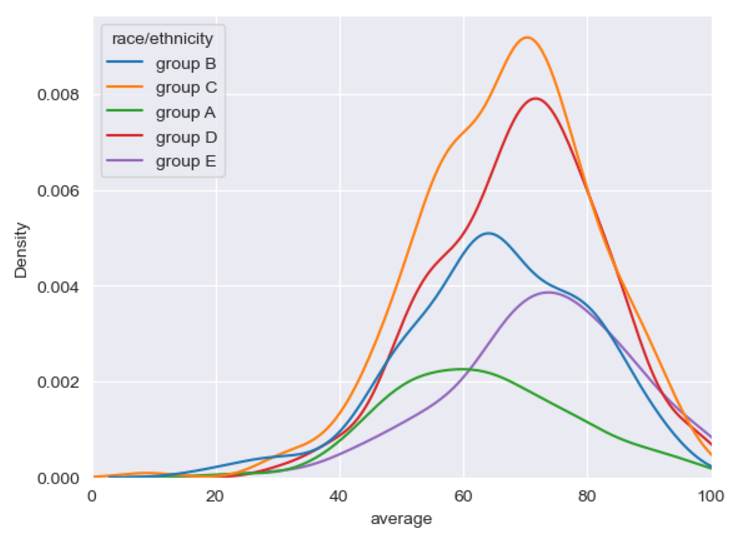
\includegraphics[width=0.5\linewidth]{RaceScoreDistribution.png}
    \caption{Score Distribution Grouped By Race/Ethnicity}
    \label{fig:RaceScores}
\end{figure}

Lastly we looked at participation in a test preparation program and student success.  A test preparation program can also be a proxy for student socioeconomic status given most of these programs cost a significant amount of money, precluding lower socioeconomic status students from participating.
Looking at the dataset split on participation in one of these test preparation courses, it is completely opposite the lunch plan differential. About two thirds of the students in the dataset did not participate in a test preparation course.  Those who did, however, saw improvements across all three test subjects.

\begin{figure}[H]
    \centering
    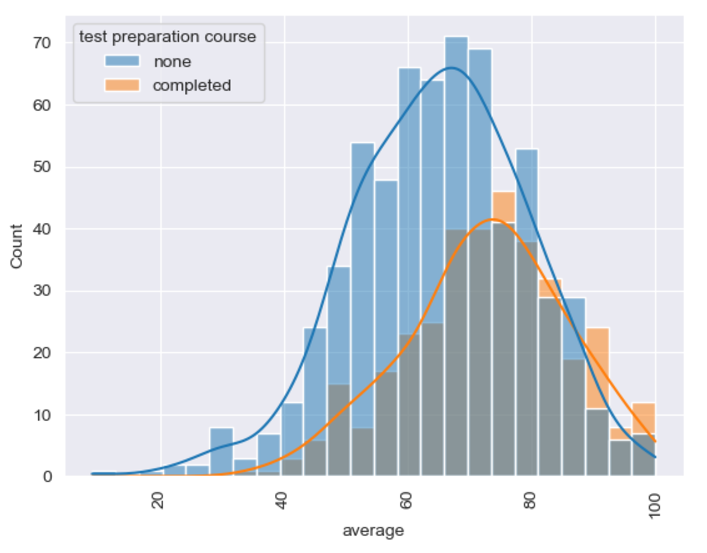
\includegraphics[width=0.75\linewidth]{TestPrepOverall.png}
    \caption{Participation in Test Prep Course Score Outcome}
    \label{fig:TestPrepOverall}
\end{figure}
Students who were able to complete a Test Preparation Program saw an overall average score 10 points higher than their counterparts. More significantly, the difference between the two means was across the passing mark. Students who were able to complete one of these courses were significantly more likely to have passed all three assessments.

\begin{figure}[H]
    \centering
    \caption{Test Preparation Course Participation vs Student Outcomes}
    \begin{subfigure}[b]{0.25\textwidth}
        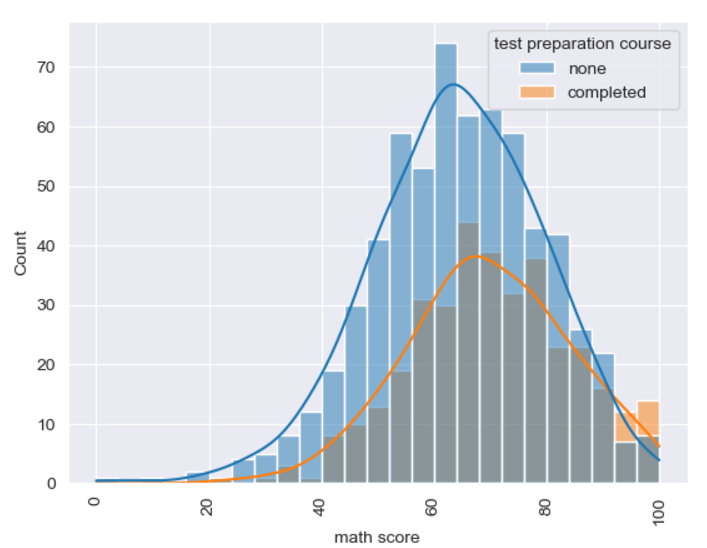
\includegraphics[width=\linewidth]{TestPrepMath.png}
        \caption{Test Prep vs. Math Scores}
        \label{fig:TestPrepMath}
    \end{subfigure}
    \begin{subfigure}[b]{0.25\textwidth}
        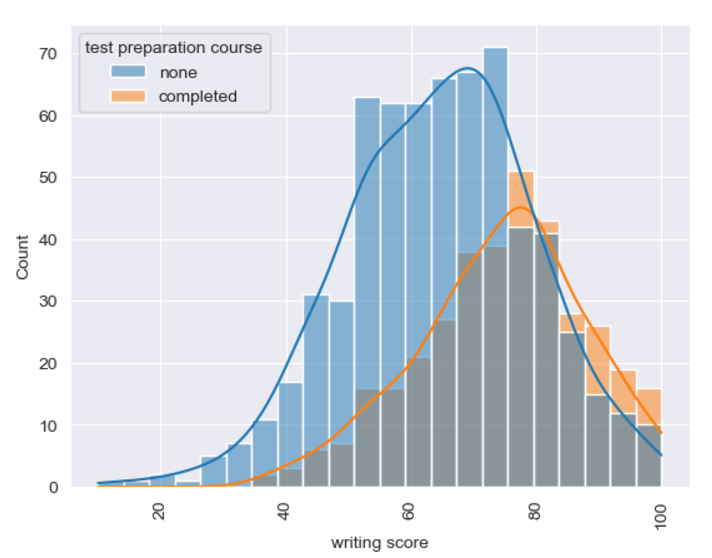
\includegraphics[width=\linewidth]{TestPrepWriting.png}
        \caption{Test Prep vs. Writing Scores}
        \label{fig:TestPrepMath}
    \end{subfigure}
    \begin{subfigure}[b]{0.25\textwidth}
        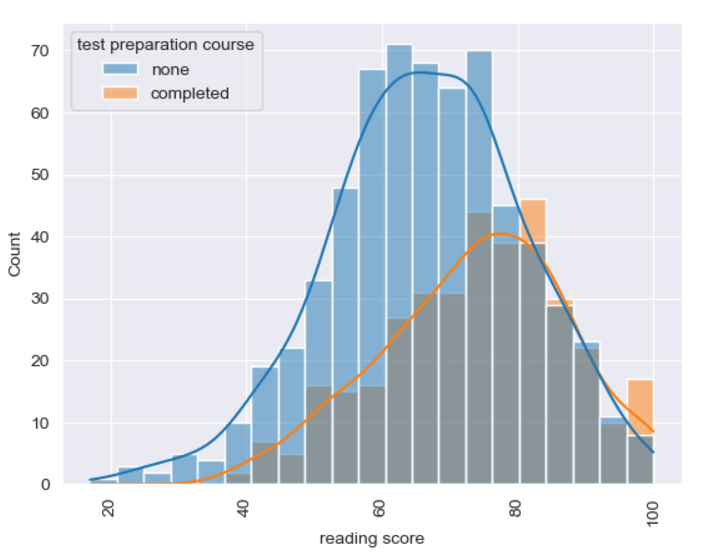
\includegraphics[width=\linewidth]{TestPrepReading.png}
        \caption{Test Prep vs. Reading Scores}
        \label{fig:TestPrepRead}
    \end{subfigure}
\end{figure}
When looking at specific subjects, Math scores showed the least improvement from a test preparation course, while Reading and Writing scores showed rather significant improvements.  Once again this is an indicator that family socioeconomic status plays a significant role in student outcomes. A family which is able to afford these programs provides yet another resources for their students to succeed while those whose families cannot afford it may be retained in grade or simply passed forward with fewer of the skills to be successful in future academic endeavors.

\subsection{Data Preparation}
The chosen dataset \cite{dataset} is a generated dataset. It is not real student information, but created to replicate a student database.  It consists of 8 columns, representing the following data.  The second column denotes valid values for that category.
\begin{table}[H]
    \centering
    \begin{tabular}{|l|p{8cm}|}
    \hline
        Gender & female/male\\
        \hline
        Race/Ethnicity & Group (A/B/C/D/E)\\
        \hline
        Parental Level of Education & Some High School, High School, Some College, Associate's Degree, Bachelor's Degree, Master's Degree\\
        \hline
        Lunch Program & Reduced/Free or None\\
        \hline
        Test Preparation Course & None/Completed\\
        \hline
        Math Assessment Score & Numeric from 0 to 100\\
        \hline
        Reading Assessment Score & Numeric from 0 to 100\\
        \hline
        Writing Assessment Score & Numeric from 0 to 100\\
        \hline
    \end{tabular}
    \caption{Columns from Student Performance in Exams Dataset}
    \label{tab:datasetCol}
\end{table}

The dataset is fairly evenly split between male and female students, skewing slightly more female at 52\% of the inputs. Students on the reduced/free lunch program make up about 1/3 of the dataset inputs, while those who completed a test preparation course also make up 1/3 of the dataset students. Race/ethnicity groups are broken up by group value, not by specific identity. Group C is the largest representative group with 319 students, with Group A being the smallest with 89 students. Investigating the cross population of these racial groups with the available socioeconomic status could provide significant insights into which students require the most assistance to be successful, or other systemic issues holding these students back.

\section{Results and Analysis}
The initial attempt used a simple Sequential model made of keras layers. The first model consisted of three Dense layers where the first layer produced a [64]  output with a sigmoid activation, the second layer a [32] output with a softmax activation, and the final layer a single [1] prediction value between 0 and 100 for the individual test score.  This model was tested with the following optimizers: Adam, MSE, and RMSProp. It was also tested with the following loss functions: MSE and Binary Crossentropy. All combinations were attempted for best accuracy. The best combination was RMSProp with Binary Crossentropy. The model was evaluated across math, writing, and reading, individually, and the accuracy was fairly close in all cases. Accuracy ranged from 63 to 65 percent across all three metrics individually.  Increasing the number of epochs did not significantly increase the accuracy rating.  Tuning of hyperparameters had a negative effect on accuracy, causing it to dip as low as 12 percent.  However, no options increased the accuracy rating with this model and best combination of optimizer/loss functions.

The next model tested was LinearRegression. The original preprocessed dataset did not perform well at all with this model. Only once MinMaxScaler was applied to normalize the dataset was the model successful at predicting the student standardized score. The metric used to evaluate the model was Mean Square Error, as 


\section{Conclusion}

\section{References}
\bibliographystyle{apacite} % APA citation style
\bibliography{bibliography}  % Reference to your .bib file

\end{document}